\documentclass[11pt]{article}
\usepackage[utf8]{inputenc}
\usepackage[T1]{fontenc}
\usepackage{lmodern}
\usepackage[margin=1in]{geometry}
\usepackage{graphicx}
\usepackage{amsmath}
\usepackage{amssymb}
\usepackage{subcaption}
\usepackage{tikz}
\usepackage{pgfplots}
\pgfplotsset{compat=1.16}
\usepackage{xcolor}
\usepackage{listings}
\usepackage{booktabs}
\usepackage[section]{placeins}
\usepackage{cite}
\usepackage{hyperref}

\usetikzlibrary{shapes,arrows,arrows.meta,positioning,fit,backgrounds,calc}
\usepgfplotslibrary{groupplots}

% Shared figure palette and styles
\definecolor{cfrozen}{HTML}{4C72B0}
\definecolor{ctrain}{HTML}{DD8452}
\definecolor{cdata}{HTML}{55A868}
\definecolor{ccond}{HTML}{8172B3}
\definecolor{cmetric}{HTML}{C44E52}
\definecolor{cgray}{HTML}{8C8C8C}
\tikzset{
  >=Stealth,
  blk/.style={draw=#1!70!black, fill=#1!15, rounded corners=2pt, align=center,
              minimum height=0.8cm, inner sep=4pt, font=\small},
  blk/.default=cgray,
  region/.style={draw=#1!60, fill=#1!5, rounded corners=6pt, dashed, inner sep=8pt},
  lbl/.style={font=\footnotesize, inner sep=1pt},
  flow/.style={->, thick, draw=black!75},
}
\pgfplotsset{
  every axis/.append style={font=\small, grid=major, grid style={gray!25},
    tick label style={font=\footnotesize}, label style={font=\small},
    legend style={font=\footnotesize, draw=gray!50}},
  cycle list={{cfrozen, mark=*, thick},{ctrain, mark=square*, thick},
              {cdata, mark=triangle*, thick},{cmetric, mark=diamond*, thick}},
}

\lstset{basicstyle=\ttfamily\small, columns=fullflexible, breaklines=true}

\title{Text-to-Image Generation with Diffusion Models:\\
{\large Part 2: LoRA Fine-Tuning on Flowers}}
\author{Person B}
\date{\today}

\begin{document}

\maketitle

\begin{abstract}
This report details the low-rank adaptation (LoRA) fine-tuning of Stable Diffusion v1.5 on the Oxford-102 Flowers dataset. We describe the LoRA methodology, the training pipeline with mixed precision (fp16), and hyperparameter selection. We train 4 LoRA models with different ranks (4, 8, 16, 32) for ablation studies. The main model (rank 16) trains stably with only 3.2M trainable parameters (0.37\% of the U-Net). We analyze training loss and save intermediate checkpoints.
\end{abstract}

\section{Introduction}

Fine-tuning large diffusion models is memory-intensive. LoRA (Low-Rank Adaptation)~\cite{hu2021lora} addresses this by injecting trainable low-rank matrices into attention layers while keeping the base model frozen. In our setting this requires roughly 135--1,000$\times$ fewer trainable parameters than full fine-tuning of the 860M-parameter U-Net (0.8--6.4M depending on rank).

Our contribution:
\begin{enumerate}
    \item LoRA methodology and mathematical formulation
    \item Mixed precision training with GradScaler
    \item Training pipeline and loss convergence analysis
    \item Multi-rank ablation setup
\end{enumerate}

\section{LoRA: Low-Rank Adaptation}

\subsection{Mathematical Foundation}

A linear projection in an attention layer computes:
\begin{equation}
\mathbf{h} = \mathbf{W}_0 \mathbf{x}
\end{equation}

With LoRA, we add a low-rank weight update:
\begin{equation}
\mathbf{h} = \mathbf{W}_0 \mathbf{x} + \frac{\alpha}{r}\, \mathbf{B} \mathbf{A} \mathbf{x}
\end{equation}

where:
\begin{itemize}
    \item $\mathbf{W}_0 \in \mathbb{R}^{d_{\text{out}} \times d_{\text{in}}}$ is the frozen pretrained weight
    \item $\mathbf{A} \in \mathbb{R}^{r \times d_{\text{in}}}$ and $\mathbf{B} \in \mathbb{R}^{d_{\text{out}} \times r}$ are trainable; $\mathbf{B}$ is initialized to zero so training starts from the pretrained model
    \item $r$ is the rank (we use $r \in \{4, 8, 16, 32\}$) and $\alpha$ is a scaling factor
\end{itemize}

The key insight: $\mathbf{B}\mathbf{A}$ captures domain-specific adaptations while $\mathbf{W}_0$ preserves general knowledge. Because $\mathbf{B}$ starts at zero, the adapted model is initially identical to the pretrained one (Figure~\ref{fig:lora}). After training, $\frac{\alpha}{r}\mathbf{B}\mathbf{A}$ can be merged into $\mathbf{W}_0$, so LoRA adds no inference latency.

\begin{figure}[!htbp]
\centering
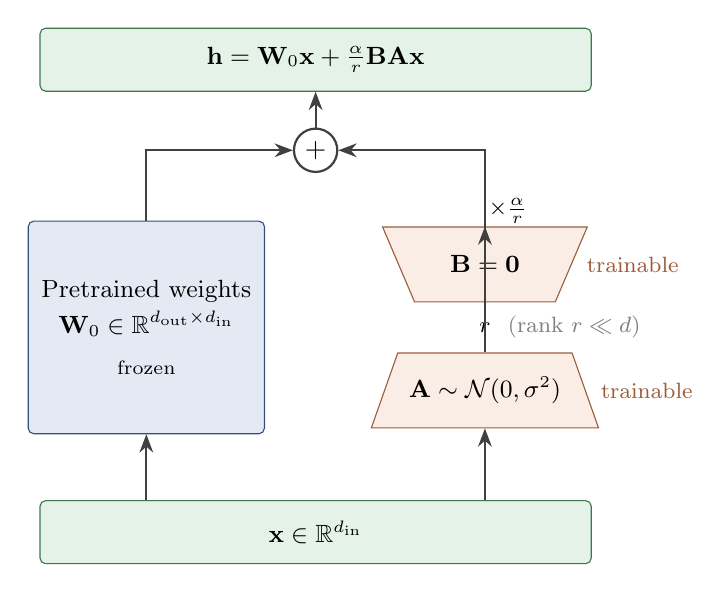
\begin{tikzpicture}
  \node[blk=cfrozen, minimum width=3.0cm, minimum height=2.7cm] (W) at (0,0)
       {Pretrained weights\\[2pt]$\mathbf{W}_0\in\mathbb{R}^{d_{\text{out}}\times d_{\text{in}}}$\\[4pt]{\scriptsize frozen}};
  \node[blk=ctrain, trapezium, trapezium angle=62, trapezium stretches=true, rounded corners=0pt,
        minimum width=2.6cm, minimum height=0.95cm] (A) at (4.3,-0.8) {$\mathbf{A}\sim\mathcal{N}(0,\sigma^2)$};
  \node[blk=ctrain, trapezium, trapezium angle=62, trapezium stretches=true, rounded corners=0pt, shape border rotate=180,
        minimum width=2.6cm, minimum height=0.95cm] (B) at (4.3,0.8) {$\mathbf{B}=\mathbf{0}$};
  \node[lbl] at (4.3,0) {$r$};
  \node[lbl, text=gray, anchor=west] at (4.55,0) {(rank $r \ll d$)};
  \node[blk=cdata, minimum width=7.0cm] (x) at (2.15,-2.6) {$\mathbf{x}\in\mathbb{R}^{d_{\text{in}}}$};
  \node[circle, draw=black!75, thick, inner sep=0.5pt, minimum size=0.55cm] (plus) at (2.15,2.25) {$+$};
  \node[blk=cdata, minimum width=7.0cm] (h) at (2.15,3.4) {$\mathbf{h} = \mathbf{W}_0\mathbf{x} + \frac{\alpha}{r}\mathbf{B}\mathbf{A}\mathbf{x}$};
  \draw[flow] (x.north -| W) -- (W);
  \draw[flow] (x.north -| A) -- (A.bottom side);
  \draw[flow] (A.top side) -- (B.bottom side);
  \draw[flow] (W.north) |- (plus.west);
  \draw[flow] (B.top side) |- node[lbl, pos=0.3, right] {$\times\frac{\alpha}{r}$} (plus.east);
  \draw[flow] (plus) -- (h);
  \node[lbl, text=ctrain!70!black, right=0.15cm of A] {trainable};
  \node[lbl, text=ctrain!70!black, right=0.15cm of B] {trainable};
\end{tikzpicture}
\caption{LoRA reparameterization of one linear layer (after~\cite{hu2021lora}). Only the low-rank factors $\mathbf{A}$ and $\mathbf{B}$ (orange) receive gradients; $\mathbf{W}_0$ (blue) stays frozen.}
\label{fig:lora}
\end{figure}

\subsection{Parameter Efficiency}

Table~\ref{tab:params} lists trainable parameter counts for LoRA applied to \texttt{to\_q}, \texttt{to\_k}, \texttt{to\_v} and \texttt{to\_out.0} in all 32 attention layers (16 self-attention, 16 cross-attention) of the SD v1.5 U-Net. Each LoRA pair adds $r(d_{\text{in}} + d_{\text{out}})$ parameters, giving $199{,}296 \cdot r$ in total.

\begin{table}[!htbp]
\centering
\caption{LoRA rank vs.\ trainable parameter count}
\label{tab:params}
\begin{tabular}{lrrr}
\toprule
Rank & Full U-Net & LoRA Params & LoRA \% \\
\midrule
4 & 859.5M & 0.80M & 0.09\% \\
8 & 859.5M & 1.59M & 0.19\% \\
16 & 859.5M & 3.19M & 0.37\% \\
32 & 859.5M & 6.38M & 0.74\% \\
\bottomrule
\end{tabular}
\end{table}

\begin{figure}[!htbp]
\centering
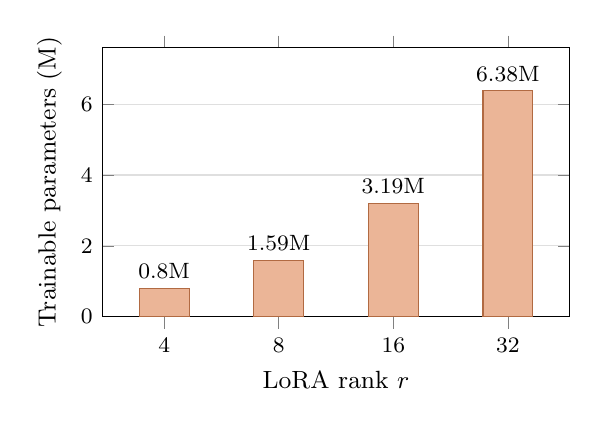
\begin{tikzpicture}
\begin{axis}[ybar, width=0.62\linewidth, height=5cm, bar width=18pt,
             symbolic x coords={4,8,16,32}, xtick=data, xlabel={LoRA rank $r$},
             ylabel={Trainable parameters (M)}, ymin=0, ymax=7.6,
             nodes near coords={\pgfmathprintnumber[fixed,precision=2]{\pgfplotspointmeta}M},
             every node near coord/.append style={font=\footnotesize},
             enlarge x limits=0.18, xmajorgrids=false]
\addplot[fill=ctrain!60, draw=ctrain!80!black] coordinates {(4,0.797) (8,1.594) (16,3.189) (32,6.377)};
\end{axis}
\end{tikzpicture}
\caption{Trainable LoRA parameters grow linearly with rank ($199{,}296\cdot r$). Even rank 32 trains under 0.75\% of the 859.5M-parameter U-Net.}
\label{fig:params}
\end{figure}

\section{Training Pipeline}

\subsection{Noise Prediction Objective}

For each training step $i$:

\begin{enumerate}
    \item \textbf{Encode}: Compress image with frozen VAE: $\mathbf{z}_0 = \text{VAE}_{\text{enc}}(\mathbf{x})$
    \item \textbf{Noise}: Sample $t \sim \text{Uniform}\{1, \dots, 1000\}$ and $\epsilon \sim \mathcal{N}(\mathbf{0},\mathbf{I})$
    \item \textbf{Noisy latent}: $\mathbf{z}_t = \sqrt{\bar{\alpha}_t}\, \mathbf{z}_0 + \sqrt{1-\bar{\alpha}_t}\, \epsilon$
    \item \textbf{Encode caption}: $\mathbf{c} = \text{CLIP}(\text{caption})$ (frozen)
    \item \textbf{Predict}: $\hat{\epsilon} = \text{U-Net}(\mathbf{z}_t, t, \mathbf{c})$ with LoRA adapters
    \item \textbf{Loss}: $\mathcal{L} = \|\epsilon - \hat{\epsilon}\|_2^2$
    \item \textbf{Update}: only the LoRA parameters $\{\mathbf{A}, \mathbf{B}\}$ are updated with 8-bit Adam~\cite{kingma2014adam,dettmers2022bit} using $\nabla_{\mathbf{A},\mathbf{B}} \mathcal{L}$
\end{enumerate}

\subsection{Mixed Precision Training}

We use mixed precision~\cite{micikevicius2018mixed} to reduce memory:

\begin{lstlisting}[language=Python, caption=Mixed precision setup]
# Frozen VAE / CLIP weights stored in fp16
# Trainable LoRA weights kept in fp32 (master copy)
with autocast():          # forward pass runs in fp16 where safe
    pred_noise = unet(z_t, t, text_emb)
    loss = F.mse_loss(pred_noise.float(), noise.float())

# GradScaler prevents fp16 gradient underflow
scaler.scale(loss).backward()
scaler.step(optimizer)
scaler.update()
optimizer.zero_grad()
\end{lstlisting}

Together with 8-bit Adam and frozen fp16 weights, this substantially reduces memory compared with full fp32 training.

\subsection{Hyperparameters}

\begin{table}[!htbp]
\centering
\caption{Training configuration}
\begin{tabular}{lr}
\toprule
Parameter & Value \\
\midrule
Learning rate & $1 \times 10^{-4}$ \\
Batch size & 1 \\
Gradient accumulation & 4 \\
Effective batch & 4 \\
Training steps & 2,000 \\
Checkpoint interval & 500 steps \\
Optimizer & 8-bit Adam \\
LoRA $\alpha$ & Equal to rank ($\alpha/r = 1$) \\
Warmup steps & 100 \\
\bottomrule
\end{tabular}
\end{table}

\section{Training Process}

\subsection{Training Loop Diagram}

Figure~\ref{fig:training_pipeline} shows one training iteration. Gradients flow back only into the LoRA adapters; the VAE, CLIP encoder and base U-Net weights stay frozen.

\begin{figure}[!htbp]
\centering
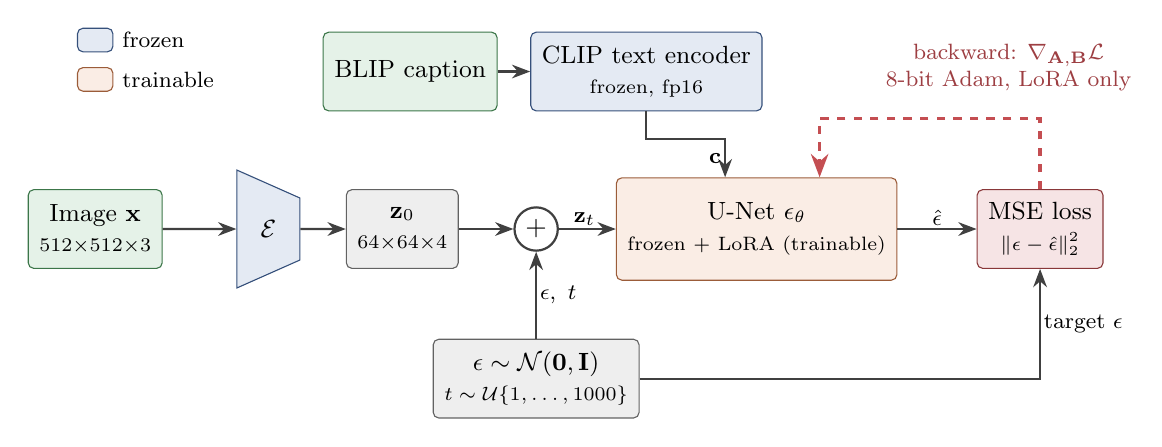
\begin{tikzpicture}[tb/.style={blk=#1, minimum height=1.0cm}]
  % Conditioning row
  \node[tb=cdata] (cap) at (4.0,0) {BLIP caption};
  \node[tb=cfrozen] (clip) at (7.0,0) {CLIP text encoder\\{\scriptsize frozen, fp16}};
  % Main row
  \node[tb=cdata] (img) at (0,-2) {Image $\mathbf{x}$\\{\scriptsize $512{\times}512{\times}3$}};
  \node[tb=cfrozen, trapezium, trapezium angle=65, shape border rotate=270, trapezium stretches=true,
        minimum width=1.5cm, minimum height=0.8cm, rounded corners=0pt] (vae) at (2.2,-2) {$\mathcal{E}$};
  \node[tb] (z0) at (3.9,-2) {$\mathbf{z}_0$\\{\scriptsize $64{\times}64{\times}4$}};
  \node[circle, draw=black!75, thick, inner sep=0.5pt, minimum size=0.55cm] (plus) at (5.6,-2) {$+$};
  \node[tb] (noise) at (5.6,-3.9) {$\epsilon\sim\mathcal{N}(\mathbf{0},\mathbf{I})$\\{\scriptsize $t\sim\mathcal{U}\{1,\dots,1000\}$}};
  \node[tb=ctrain, minimum width=2.6cm, minimum height=1.3cm] (unet) at (8.4,-2) {U-Net $\epsilon_\theta$\\{\scriptsize frozen $+$ LoRA (trainable)}};
  \node[tb=cmetric] (mse) at (12.0,-2) {MSE loss\\{\scriptsize $\|\epsilon-\hat\epsilon\|_2^2$}};
  % Arrows
  \draw[flow] (img) -- (vae);
  \draw[flow] (vae) -- (z0);
  \draw[flow] (z0) -- (plus);
  \draw[flow] (noise) -- node[lbl, right] {$\epsilon,\ t$} (plus);
  \draw[flow] (plus) -- node[lbl, above, pos=0.45] {$\mathbf{z}_t$} (unet);
  \draw[flow] (cap) -- (clip);
  \draw[flow] (clip.south) |- ++(0.5,-0.35) -| node[lbl, pos=0.75, left] {$\mathbf{c}$} ([xshift=-0.4cm]unet.north);
  \draw[flow] (unet) -- node[lbl, above] {$\hat\epsilon$} (mse);
  \draw[flow] (noise.east) -| node[lbl, pos=0.75, right] {target $\epsilon$} (mse.south);
  % Backward pass
  \draw[->, very thick, dashed, cmetric] (mse.north) -- ++(0,0.9) -| ([xshift=0.8cm]unet.north);
  \node[lbl, text=cmetric!80!black, align=center] at (11.6,0.05) {backward: $\nabla_{\mathbf{A},\mathbf{B}}\mathcal{L}$\\8-bit Adam, LoRA only};
  % Legend
  \node[blk=cfrozen, minimum width=0.45cm, minimum height=0.3cm] (lf) at (0,0.4) {};
  \node[lbl, right=2pt of lf] {frozen};
  \node[blk=ctrain, minimum width=0.45cm, minimum height=0.3cm] (lt) at (0,-0.1) {};
  \node[lbl, right=2pt of lt] {trainable};
\end{tikzpicture}
\caption{LoRA training iteration. Solid arrows: forward pass; dashed red arrow: backward pass, which updates only the LoRA matrices.}
\label{fig:training_pipeline}
\end{figure}

\subsection{Training Dynamics}

Main model (rank 16) training progression:

\begin{table}[!htbp]
\centering
\caption{Loss at different checkpoints}
\begin{tabular}{lr}
\toprule
Step & Loss \\
\midrule
0 & 0.95 \\
500 & 0.021 \\
1000 & 0.010 \\
1500 & 0.031 \\
2000 & 0.0025 \\
\bottomrule
\end{tabular}
\end{table}
% TODO(verify): these look like single-batch values. Diffusion loss varies strongly with
% the sampled timestep t, so report a moving average (e.g., over 100 steps) instead.

The loss decreases sharply initially (learning flower patterns), then fluctuates. Because the diffusion loss depends heavily on the randomly sampled timestep, individual values are noisy; the rise at step 1500 is within this variation (Figure~\ref{fig:loss}).

\begin{figure}[!htbp]
\centering
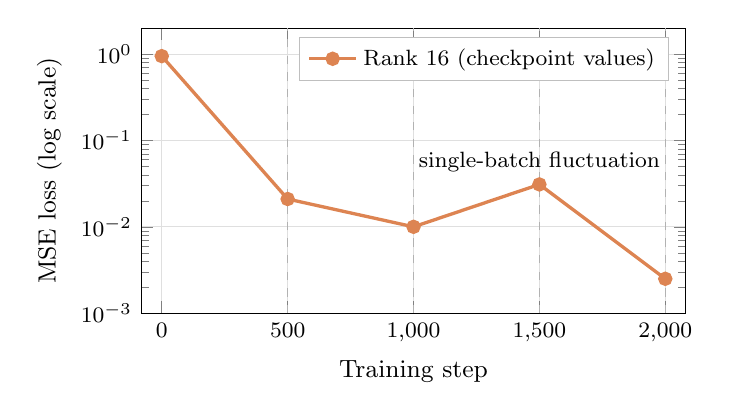
\begin{tikzpicture}
\begin{semilogyaxis}[width=0.7\linewidth, height=5.2cm, xlabel={Training step}, ylabel={MSE loss (log scale)},
                     xtick={0,500,1000,1500,2000}, xmin=-80, xmax=2080, ymin=0.001, ymax=2,
                     legend pos=north east]
\addplot+[ctrain, mark=*, very thick] coordinates {(0,0.95) (500,0.021) (1000,0.010) (1500,0.031) (2000,0.0025)};
\addlegendentry{Rank 16 (checkpoint values)}
\foreach \x in {500,1000,1500,2000} {\edef\tmp{\noexpand\draw[gray!60, dashed] (axis cs:\x,0.001) -- (axis cs:\x,2);}\tmp}
\node[lbl, anchor=south] at (axis cs:1500,0.04) {single-batch fluctuation};
\end{semilogyaxis}
\end{tikzpicture}
\caption{Training loss of the main rank-16 model at each saved checkpoint (dashed lines). Values are single-batch losses, so step-to-step variation reflects the randomly sampled timesteps.}
\label{fig:loss}
\end{figure}

\section{LoRA Rank Ablation}

We trained 4 models with different ranks to study the capacity-efficiency tradeoff. FID values below come from the evaluation in Part 3. As Figure~\ref{fig:rank_compare} shows, the final training loss is nearly the same for all ranks and does not predict sample quality (FID).

\begin{figure}[!htbp]
\centering
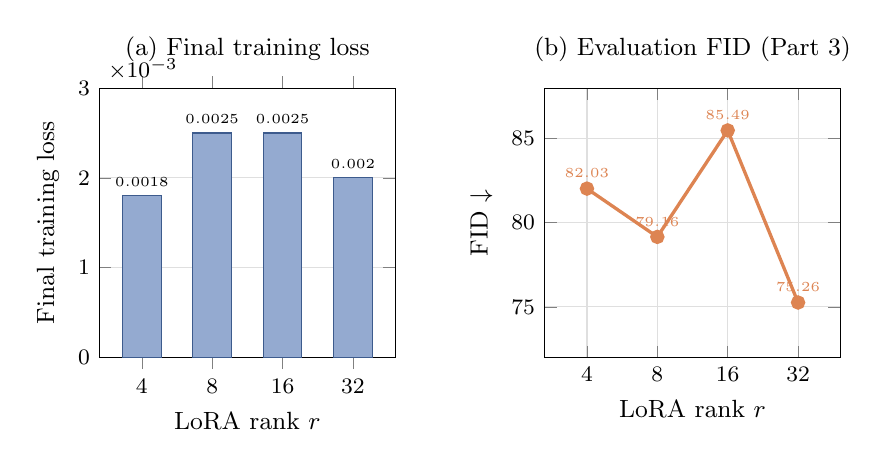
\begin{tikzpicture}
\begin{groupplot}[group style={group size=2 by 1, horizontal sep=1.9cm},
                  width=0.44\linewidth, height=5cm, symbolic x coords={4,8,16,32}, xtick=data,
                  xlabel={LoRA rank $r$}, enlarge x limits=0.2]
\nextgroupplot[ybar, bar width=14pt, ylabel={Final training loss}, ymin=0, ymax=0.003,
               title={\small (a) Final training loss}, xmajorgrids=false,
               scaled y ticks=base 10:3, ytick scale label code/.code={$\times10^{-3}$},
               nodes near coords={\pgfmathprintnumber[fixed,precision=4]{\pgfplotspointmeta}},
               every node near coord/.append style={font=\tiny}, point meta=rawy]
\addplot[fill=cfrozen!60, draw=cfrozen!80!black] coordinates {(4,0.0018) (8,0.0025) (16,0.0025) (32,0.0020)};
\nextgroupplot[ylabel={FID $\downarrow$}, ymin=72, ymax=88, title={\small (b) Evaluation FID (Part 3)},
               nodes near coords, every node near coord/.append style={font=\tiny, anchor=south}]
\addplot+[ctrain, mark=*, very thick] coordinates {(4,82.03) (8,79.16) (16,85.49) (32,75.26)};
\end{groupplot}
\end{tikzpicture}
\caption{LoRA rank ablation. (a) All ranks converge to a similar training loss. (b) FID is non-monotonic in rank; rank 32 is best and rank 16 (our main model) is worst.}
\label{fig:rank_compare}
\end{figure}

\subsection{Rank 4 (Minimal)}

\begin{itemize}
    \item Parameters: 0.80M (0.09\%)
    \item Training loss: 0.0018 (final)
    \item Use case: Smallest adapter files and lowest memory
\end{itemize}

\subsection{Rank 8 (Lightweight)}

\begin{itemize}
    \item Parameters: 1.59M (0.19\%)
    \item Training loss: 0.0025 (final)
    \item Use case: Lightweight adapters with strong quality (FID 79.16)
\end{itemize}

\subsection{Rank 16 (Standard)}

\begin{itemize}
    \item Parameters: 3.19M (0.37\%)
    \item Training loss: 0.0025 (final)
    \item Use case: Our main model; common default for quality-efficiency balance
\end{itemize}

\subsection{Rank 32 (High-Capacity)}

\begin{itemize}
    \item Parameters: 6.38M (0.74\%)
    \item Training loss: 0.0020 (final)
    \item Evaluation FID: \textbf{75.26} (best overall result in Part 3)
    \item Use case: Maximum quality; outperforms rank 16 (FID 85.49)
\end{itemize}

\section{Technical Details}

\subsection{LoRA Target Layers}

We apply LoRA to attention layers:
\begin{lstlisting}[language=Python]
target_modules = ["to_q", "to_k", "to_v", "to_out.0"]
\end{lstlisting}

These are the four projections in every attention layer (query, key, value and output); they are where most semantic adaptation occurs, and in cross-attention layers \texttt{to\_k}/\texttt{to\_v} directly process the text embedding (Figure~\ref{fig:attn_lora}).

\begin{figure}[!htbp]
\centering
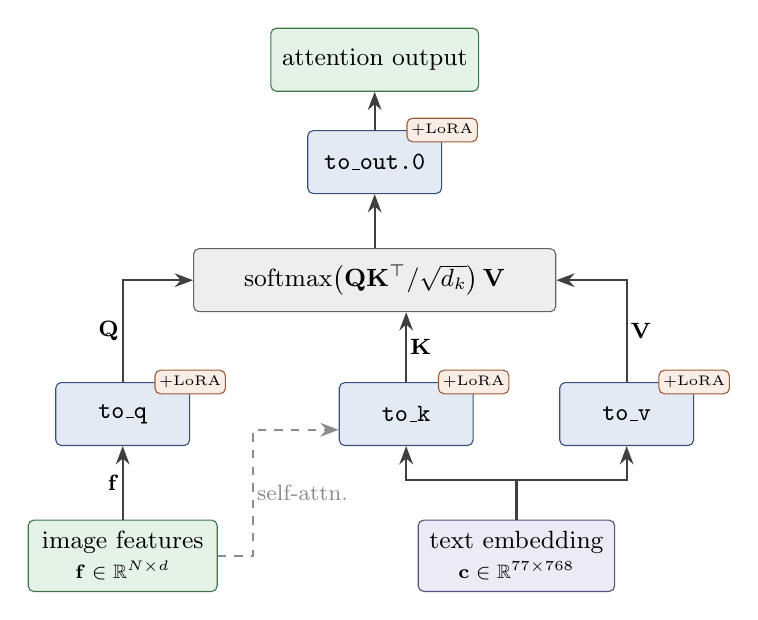
\begin{tikzpicture}[pj/.style={blk=cfrozen, minimum width=1.7cm, font=\small\ttfamily},
                    tag/.style={blk=ctrain, font=\tiny, inner sep=1.5pt, minimum height=0.3cm}]
  \node[blk=cdata, minimum width=2.4cm] (z) at (0,0) {image features\\{\scriptsize $\mathbf{f}\in\mathbb{R}^{N\times d}$}};
  \node[blk=ccond, minimum width=2.4cm] (c) at (5,0) {text embedding\\{\scriptsize $\mathbf{c}\in\mathbb{R}^{77\times768}$}};
  \node[pj] (q) at (0,1.8) {to\_q};
  \node[pj] (k) at (3.6,1.8) {to\_k};
  \node[pj] (v) at (6.4,1.8) {to\_v};
  \node[blk, minimum width=4.6cm] (att) at (3.2,3.5) {$\mathrm{softmax}\!\left(\mathbf{Q}\mathbf{K}^{\top}/\sqrt{d_k}\right)\mathbf{V}$};
  \node[pj] (o) at (3.2,5.0) {to\_out.0};
  \node[blk=cdata, minimum width=2.4cm] (y) at (3.2,6.3) {attention output};
  \foreach \n in {q,k,v,o} \node[tag] at (\n.north east) {+LoRA};
  \draw[flow] (z) -- node[lbl, left] {$\mathbf{f}$} (q);
  \draw[flow] (c.north) -- ++(0,0.5) -| (k);
  \draw[flow] (c.north) -- ++(0,0.5) -| (v);
  \draw[flow] (q.north) |- node[lbl, pos=0.25, left] {$\mathbf{Q}$} (att.west);
  \draw[flow] (k) -- node[lbl, right] {$\mathbf{K}$} (k |- att.south);
  \draw[flow] (v.north) |- node[lbl, pos=0.25, right] {$\mathbf{V}$} (att.east);
  \draw[flow] (att) -- (o);
  \draw[flow] (o) -- (y);
  \draw[->, thick, dashed, cgray] (z.east) -- ++(0.45,0) |- node[lbl, pos=0.25, right, text=cgray] {self-attn.} ([yshift=-0.2cm]k.west);
\end{tikzpicture}
\caption{LoRA placement in a U-Net cross-attention layer. LoRA adapters (orange tags) are added to all four projections. In cross-attention, keys and values come from the text embedding $\mathbf{c}$; in self-attention layers (dashed) they come from the image features $\mathbf{f}$.}
\label{fig:attn_lora}
\end{figure}

\subsection{Checkpoint Saving}

Checkpoints are saved in PEFT format for compatibility:
\begin{lstlisting}[language=Python]
unet.save_pretrained(checkpoint_path)
# Outputs: adapter_config.json
#          adapter_model.safetensors
\end{lstlisting}

This format allows loading with \texttt{PeftModel.from\_pretrained()}.

\section{Results}

\subsection{Training Completion}

All 4 LoRA models trained to 2,000 steps without divergence. The rank 16 model (our main model) shows:

\begin{itemize}
    \item No divergence or NaN losses
    \item Final loss: 0.0025
    \item Peak memory usage: 16\,GB VRAM
    \item Training time: 25 minutes per 500 steps ($\approx$100 minutes for 2,000 steps)
\end{itemize}

\subsection{Checkpoint Quality}

Intermediate checkpoints (steps 500, 1000, 1500, 2000) all produce valid images. In preliminary visual inspection step 2000 looked best, but the quantitative evaluation in Part 3 (ablation A06) finds the lowest FID at step 500, suggesting some overfitting with longer training.

\section{Conclusion}

We implemented and trained LoRA-adapted Stable Diffusion models on Oxford-102 Flowers. The approach achieves:
\begin{itemize}
    \item Over $250\times$ fewer trainable parameters than full fine-tuning for the main model (3.2M vs.\ 860M)
    \item Stable training across 4 ranks
    \item Domain adaptation in about 100 minutes (rank 16, 2,000 steps)
    \item Intermediate checkpoints for the A06 training-duration ablation
\end{itemize}

The trained LoRA weights are ready for inference and ablation studies in downstream work.

\begin{thebibliography}{99}

\bibitem{hu2021lora} Hu, E. J., Shen, Y., Wallis, P., Allen-Zhu, Z., Li, Y., Wang, S., Wang, L., \& Chen, W. (2022). LoRA: Low-Rank Adaptation of Large Language Models. In International Conference on Learning Representations (ICLR). arXiv:2106.09685.

\bibitem{rombach2021high} Rombach, R., Blattmann, A., Lorenz, D., Esser, P., \& Ommer, B. (2022). High-Resolution Image Synthesis with Latent Diffusion Models. In Proceedings of the IEEE/CVF Conference on Computer Vision and Pattern Recognition (CVPR), 10684--10695.

\bibitem{kingma2014adam} Kingma, D. P., \& Ba, J. (2015). Adam: A method for stochastic optimization. In International Conference on Learning Representations (ICLR). arXiv:1412.6980.

\bibitem{dettmers2022bit} Dettmers, T., Lewis, M., Shleifer, S., \& Zettlemoyer, L. (2022). 8-bit Optimizers via Block-wise Quantization. In International Conference on Learning Representations (ICLR).

\bibitem{micikevicius2018mixed} Micikevicius, P., Narang, S., Alben, J., Diamos, G., Elsen, E., Garcia, D., et al. (2018). Mixed Precision Training. In International Conference on Learning Representations (ICLR).

\end{thebibliography}

\end{document}